\documentclass{article}
\usepackage[final]{neurips} % ready for submission, but you have multiple options to import this
\usepackage[utf8]{inputenc} % allow utf-8 input
\usepackage[T1]{fontenc}    % use 8-bit T1 fonts
\usepackage{hyperref}       % hyperlinks
\usepackage{url}            % simple URL typesetting
\usepackage{booktabs}       % professional-quality tables
\usepackage{amsfonts}       % blackboard math symbols
\usepackage{nicefrac}       % compact symbols for 1/2, etc.
\usepackage{microtype}      % microtypography
\usepackage{xcolor}         % colors
\usepackage{graphicx}
\usepackage{subfigure}

\begin{document}

\title{Soccer Dataset Prediction and Analysis}

\author{%
    GroupID: P28
    \AND
  Abhishek Rao \\
  \texttt{arao23@ncsu.edu} \\
  \And
  Manav Divyesh Shah \\
  \texttt{mdshah5@ncsu.edu} \\
  \And
  Srimadh Vasuki Rao \\
  \texttt{svrao3@ncsu.edu}
}

\maketitle


\section{Background and Introduction}
\label{gen_inst}
Data plays an essential role in our lives today. Even in areas where its significance may not be immediately obvious, it holds great importance. A prime example of this is in the world of sports, particularly soccer/football. The modern game relies heavily on data analysis. In-depth analyses can forecast a team's performance in upcoming matches or help identify potential transfer targets for clubs. A notable case is Liverpool Football Club, whose owners utilized data analysis to pinpoint transfer candidates. As a result, the team's performance dramatically improved over a few years, leading them to become a title-winning squad. This is just one illustration of how data analysis and machine learning can be applied in soccer. In this project, we will explore some of these methods.

The project utilizes the European Soccer Database, a comprehensive collection of soccer data covering the years from 2008 to 2016. This dataset merges extensive information on European football matches, teams, and players across several major leagues. It is designed to support a wide range of analyses—from evaluating performance and identifying trends to building predictive models. The dataset incorporates information from various reputable sources to guarantee accuracy and thoroughness. By consolidating data from these sources, the European Soccer Database offers a unified and organized format that makes data retrieval and analysis much simpler.

Our project is focused on achieving two main objectives: \textbf{Predicting the outcome of a specific match} and \textbf{Identifying suitable player transfers} that address the team's weaknesses. To accomplish these goals, we conduct comprehensive exploratory data analysis (EDA). This involves examining the dataset in detail to uncover correlations and relationships between various metrics for both players and teams. By analyzing factors such as player performance statistics, team dynamics, and historical match outcomes, we aim to gain valuable insights that will inform our predictive models.

\section{Method}

\subsection{Data Selection}
This project utilizes the European soccer database which contains match data, team attributes, and player statistics from major European leagues. As of now, we are using data from 2014 to 2016 to extract insights and predict. This can easily be extended from 2008 to 2016. We have also selected the top 5 leagues in Europe, English Premier League, Spanish La Liga, German Bundesliga, Italian Serie A, and French Ligue 1.

\subsection{Dataset Structure and Components}

The European Soccer Database is organized into several interrelated tables, each focusing on specific aspects of football data. The Players table contains detailed profiles, including personal information such as age and nationality, as well as physical attributes like height and weight. The Teams table provides information on football clubs, including team names, styles of play in attack and defense. The Matches table records comprehensive match details, such as date, venue, participating teams, final scores, and in-game statistics like possession percentage and number of shots. Lastly, the Player Attributes table lists various skills and attributes of players, including passing accuracy, shooting ability, defensive prowess, and overall rating, which are essential for performance analysis and player comparison.

\subsection{Data Preprocessing}
The preprocessing phase includes several essential steps to ensure data quality and consistency. Depending on the task at hand, we need to merge various tables using unique identifiers, such as $team\_fifa\_api\_id$ or $league\_id$.

Given that this is real-world data, the dataset contains numerous \textbf{missing values}. We employed an average fill method to populate the merged tables, as this approach aids in accurately predicting match outcomes. There are various techniques for handling missing values that can be explored to observe how they affect the results. Additionally, data for players and teams has been \textbf{aggregated} to analyze their performance over multiple years.

\subsection{Data Transformation}
Here we create new features/ add new features based on home/away team, that will be useful for our end goal:

\begin{enumerate}
    \item \textbf{Team Performance Metrics:} 
    We use the average rating of the players in the team and also the potential rating of the players to create home/away team ratings which are continuous ratio attributes.
    \item \textbf{Match Outcome Encoding:} Match outcomes have been encoded into a categorical variable to simplify analysis. Home Wins are assigned a value of 1, draws a value of 0, and losses a value of -1. Match outcome is a newly created attribute, by checking the home team and away team goals and deciding the winner.
    \item \textbf{Tactical Attributes:} These contains both numerical and categorical features that show us the strategic approach of teams. Numerical metrics include build-up play characteristics, such as speed, dribbling, and passing, as well as chance creation indicators and defensive organization measures. Categorical features, such as playing style classifications and tactical approach categories, have been one-hot encoded to be used for predictions.
\end{enumerate}

\subsection{Data Mining/ Prediction Strategy}
We have correlation analysis to identify the important features for match outcome prediction. We also look at various visualizations and comparisons to see how the data is spread out and to obtain insights.

For the task of \textbf{Predicting the match outcomes}, we will be using two models Random Forest and Neural Networks. The features that are selected from the EDA and Correlation analysis can be used to predict the outcomes.

For the task of \textbf{Identifying players for transfers}, we will be classifying the player's features based on their overall
role in the team, like Creator, Finisher or Defender. We will also look at all these features to identify where the team is lacking. Players can then be filtered out based on their current forms or by using Prediction using regression/Time series based regression to identify future talents based on their performances in previous seasons.

\section{Experimental Setup}


\subsection{Implementation Details}
The project is implemented using Python, using the below data science libraries:
\begin{enumerate}
    \item Pandas for data manipulation and merging
    \item NumPy for numerical computations
    \item Seaborn for statistical visualizations
    \item Matplotlib for plotting
    \item Scikit-Learn for prediction models
\end{enumerate}

\subsection{Model Evaluation}
We will use a holistic view to compare models on their prediction for match-based outcomes. We use Precision, Recall, F1-Score, and Accuracy as our main measures to compare models.


\section{Results}
\label{others}
Through exploratory data analysis, we gain valuable insights into the dataset. Figure 1 illustrates key metrics for evaluating a player, such as vision, shooting, and passing. Notably, certain patterns emerge: metrics like standing tackles, sliding tackles, and interceptions show two peaks, suggesting some players excel in these defensive roles, while others do not. In contrast, general attributes like shooting, passing, and agility present a more typical bell curve, indicating these skills are essential for all players, regardless of their roles. These metrics are crucial for identifying players who can address weaknesses in our team, as we need to focus on specific attributes when seeking players for targeted roles.

We also gain insights into why the highest-rated players excel in their positions. Analyzing the radar plots (Figure 2), it becomes evident that top-rated players exhibit a more filled-out plot compared to those with median ratings. These higher-rated players tend to focus on all aspects of their game, which makes them invaluable to any team.

Figure 3 illustrates the various play styles teams adopt in different leagues. We can see that La Liga is a highly technical league, characterized by a greater emphasis on chance-creation passing compared to other leagues. This indicates that quality scoring opportunities are primarily generated through passes rather than crosses or other methods. In terms of buildup play speed, the Bundesliga is notably fast-paced, while Ligue 1 is slower and exhibits higher defensive pressure. The style of play in a particular league significantly influences the selection of players for a team.

We used a Random Forest Classifier and a straightforward Neural Network to predict match outcomes. Initially, we used only the home and away teams' ratings and potential for our predictions. However, after incorporating team-specific features, such as buildup play speed, both models demonstrated improved performance, as seen in the results below.

\begin{table}[htbp]
    \centering
    \caption{Comparison of Random Forest and Neural Network Results}
    \begin{tabular}{@{}lcccccc@{}}
        \toprule
        \textbf{Metric} & \textbf{Random Forest} & & \textbf{Neural Network} & \\
        \cmidrule(lr){2-3} \cmidrule(lr){4-5}
        & Accuracy & F1-Score & Accuracy & F1-Score \\
        \midrule
        Overall Accuracy & 0.4284 & 0.4135 & 0.4449 & 0.4110 \\
        \midrule
        \textbf{Class} & Precision & Recall & Precision & Recall \\
        \midrule
        Away Win & 0.47 & 0.38 & 0.46 & 0.29 \\
        Draw & 0.20 & 0.15 & 0.24 & 0.14 \\
        Home Win & 0.49 & 0.62 & 0.49 & 0.73 \\
        \midrule
        Macro Avg & 0.39 & 0.38 & 0.39 & 0.39 \\
        Weighted Avg & 0.41 & 0.43 & 0.42 & 0.44 \\
        \bottomrule
    \end{tabular}
    \label{tab:model_comparison}
\end{table}
We can see that the neural network performs better than the Random Forest Classifier, in accuracy, but considering F1 scores, both of them are very similar.


\begin{figure}
    \centering
    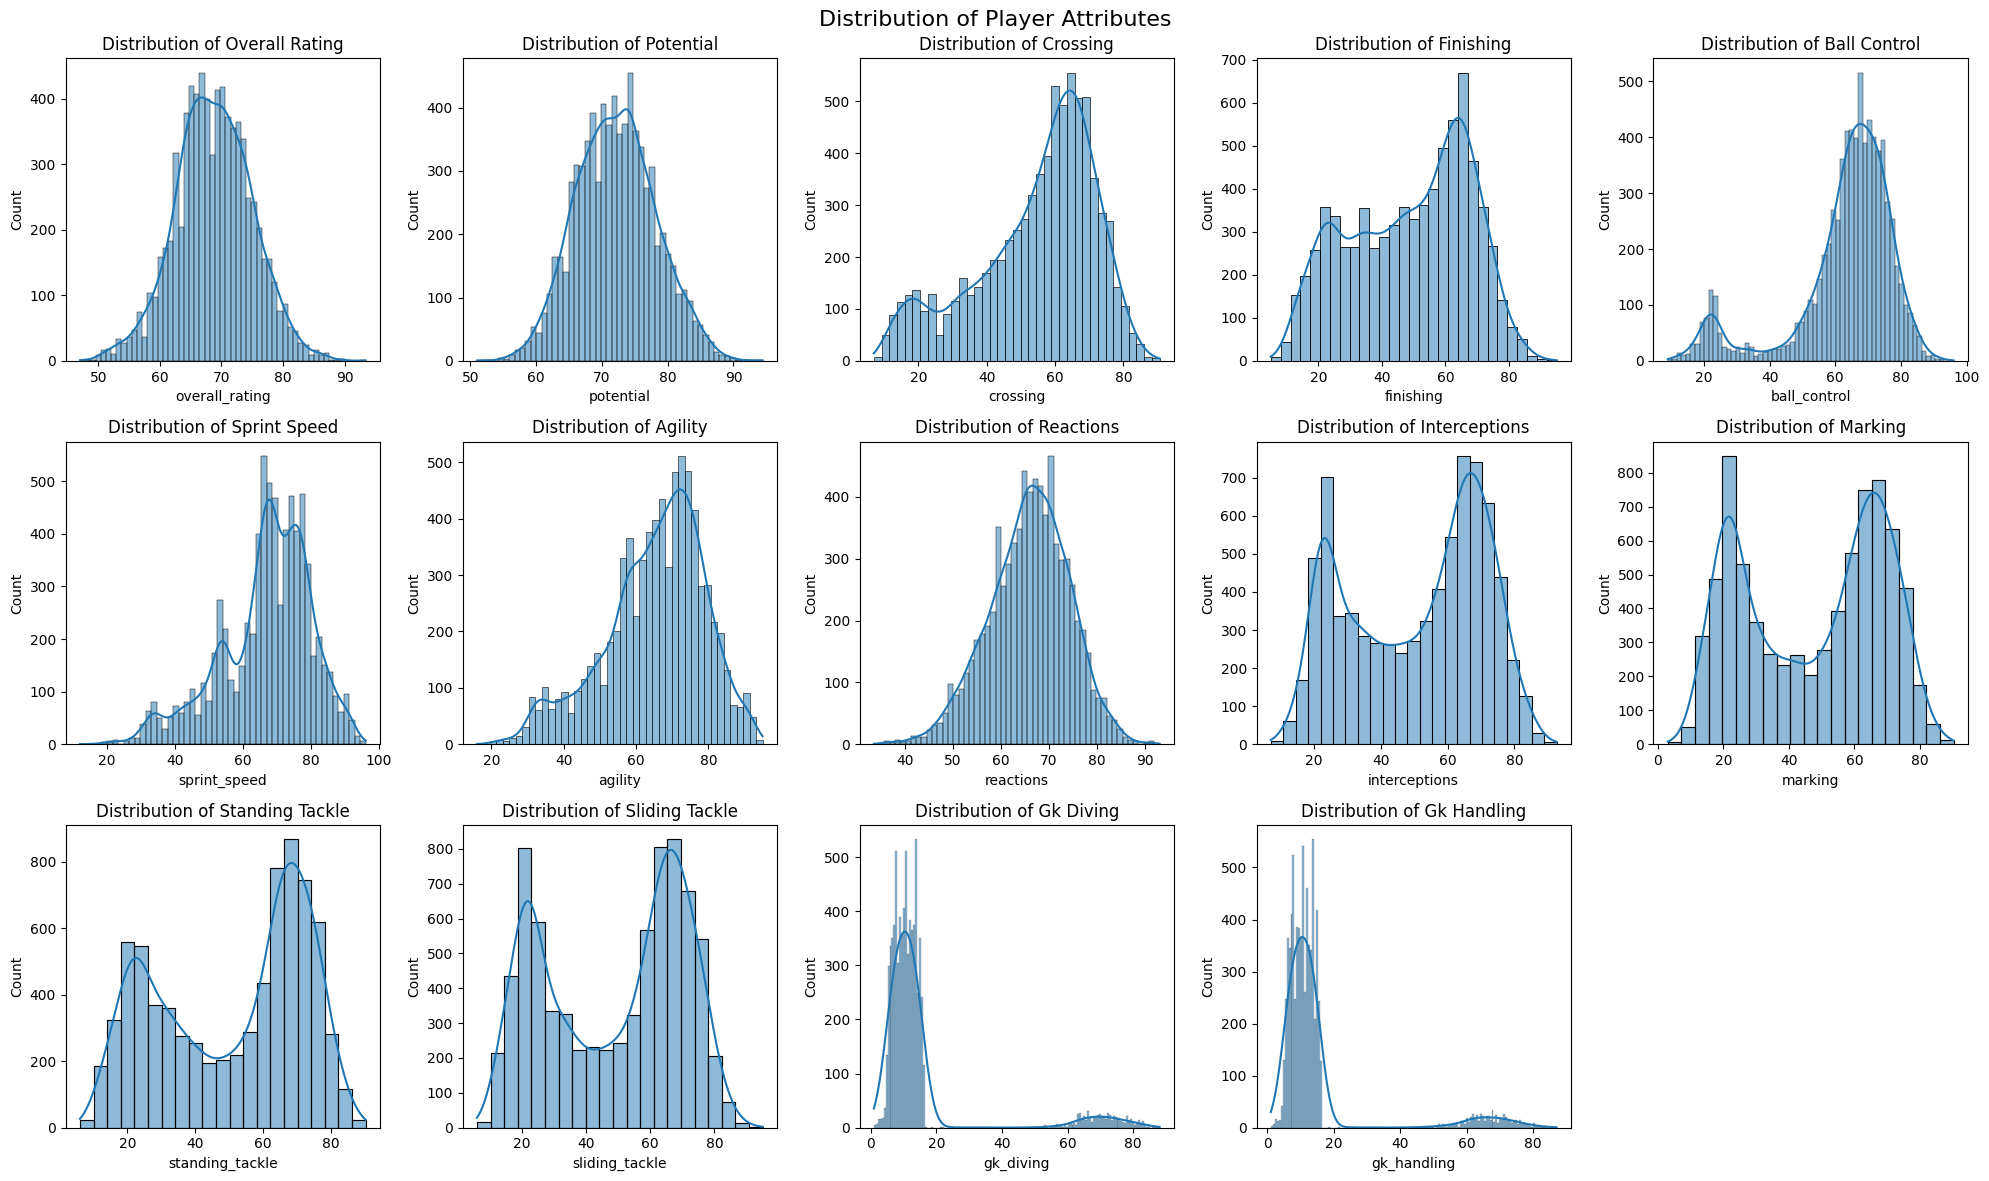
\includegraphics[width=1\linewidth]{PlayerSkills.png}
    \caption{Skill Distributions}
    \label{fig:enter-label}
\end{figure}

\begin{figure}
    \centering
    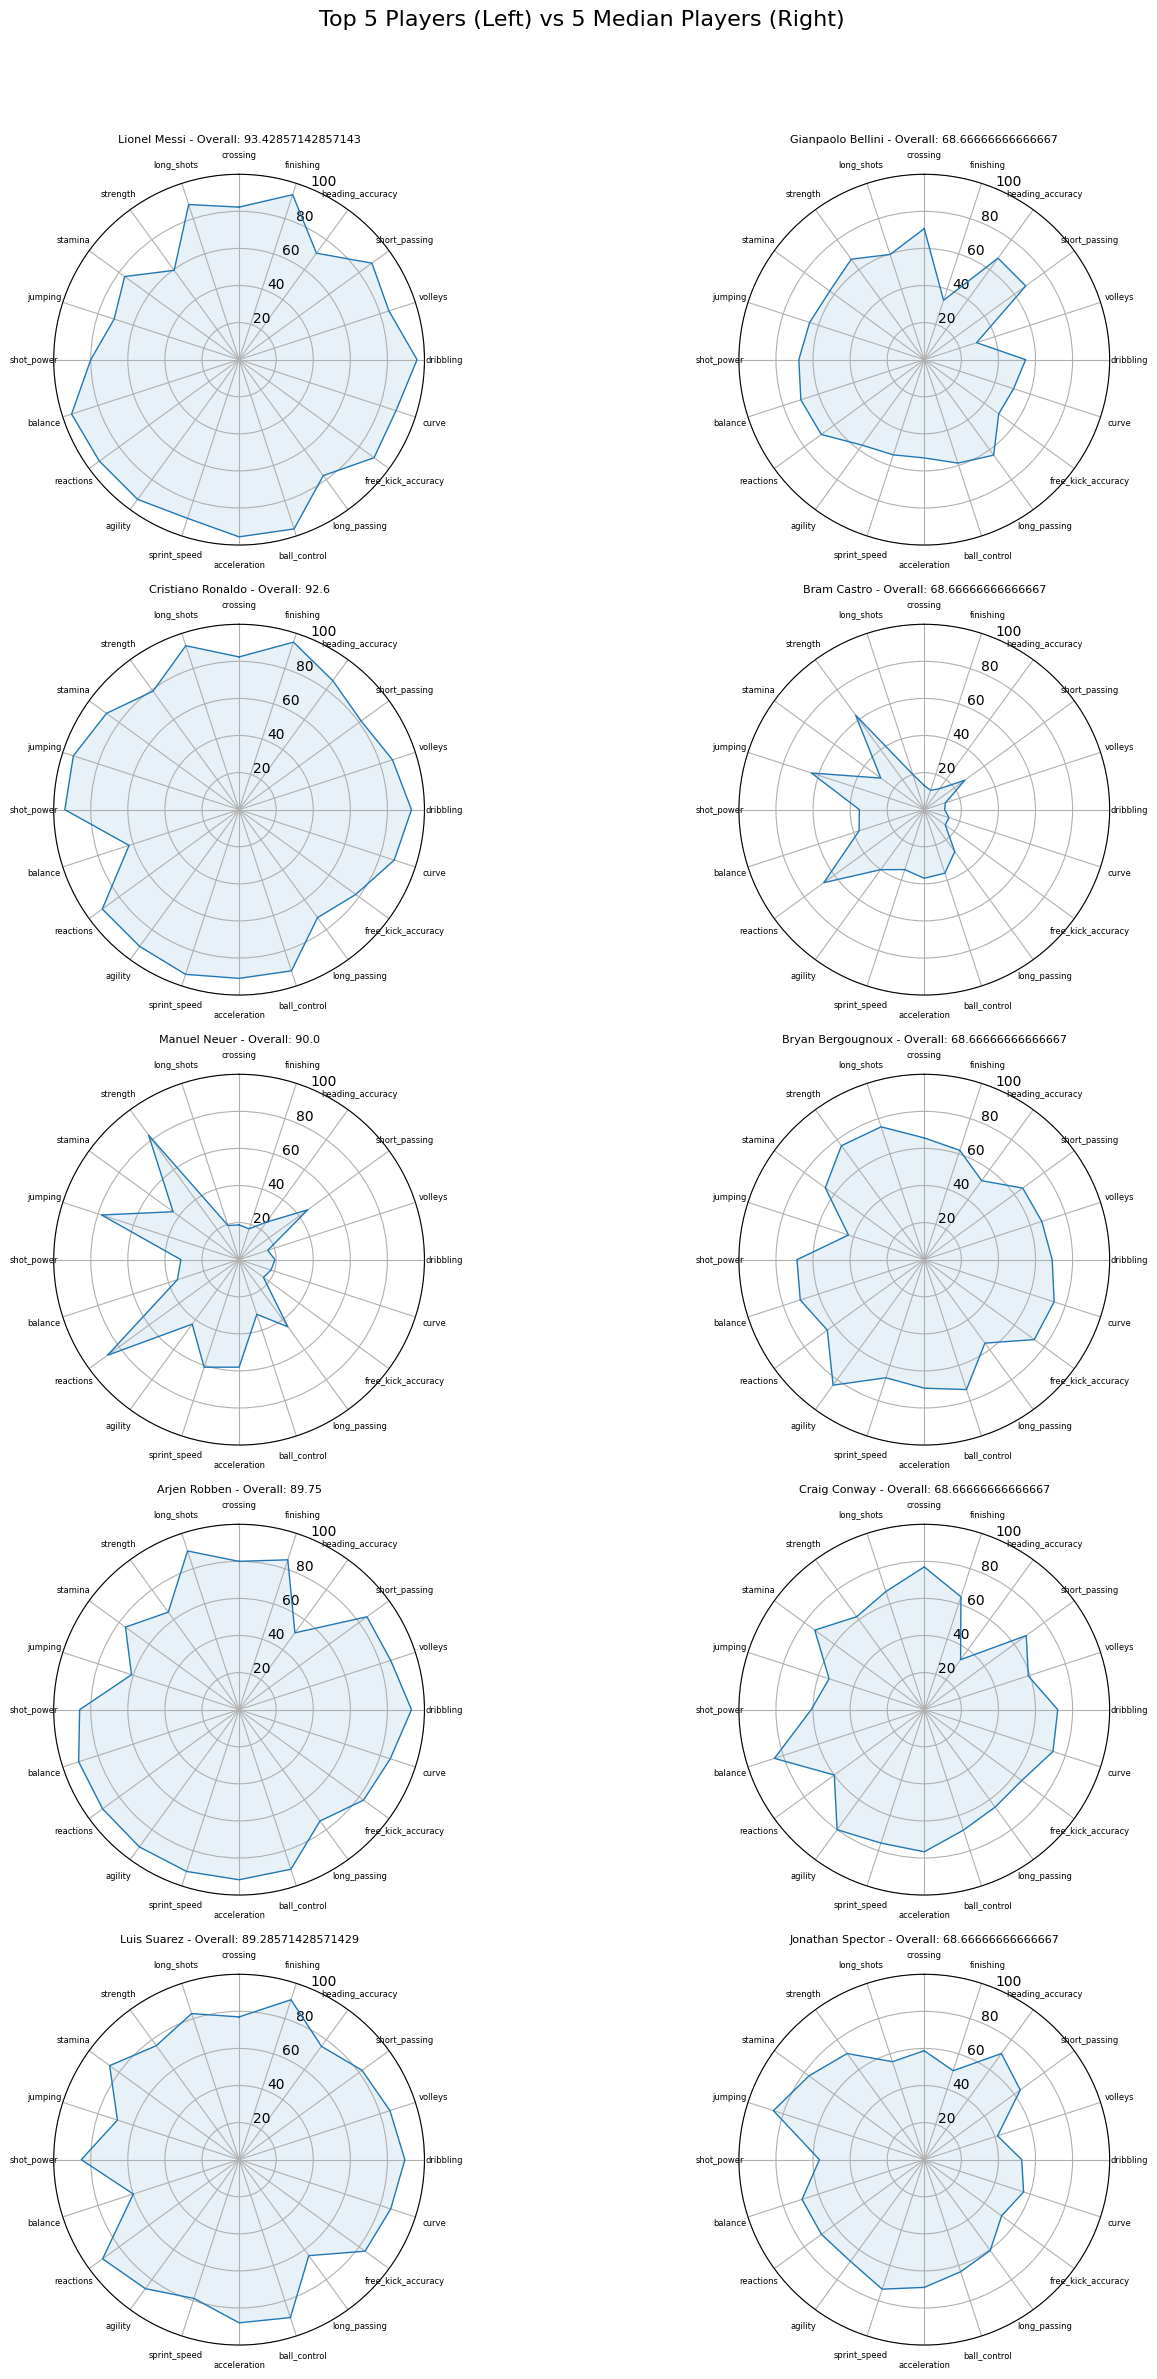
\includegraphics[width=0.4\linewidth]{top_players.png}
    \caption{Top Players V/s Median Players}
    \label{fig:enter-label}
\end{figure}

\begin{figure}
    \centering
    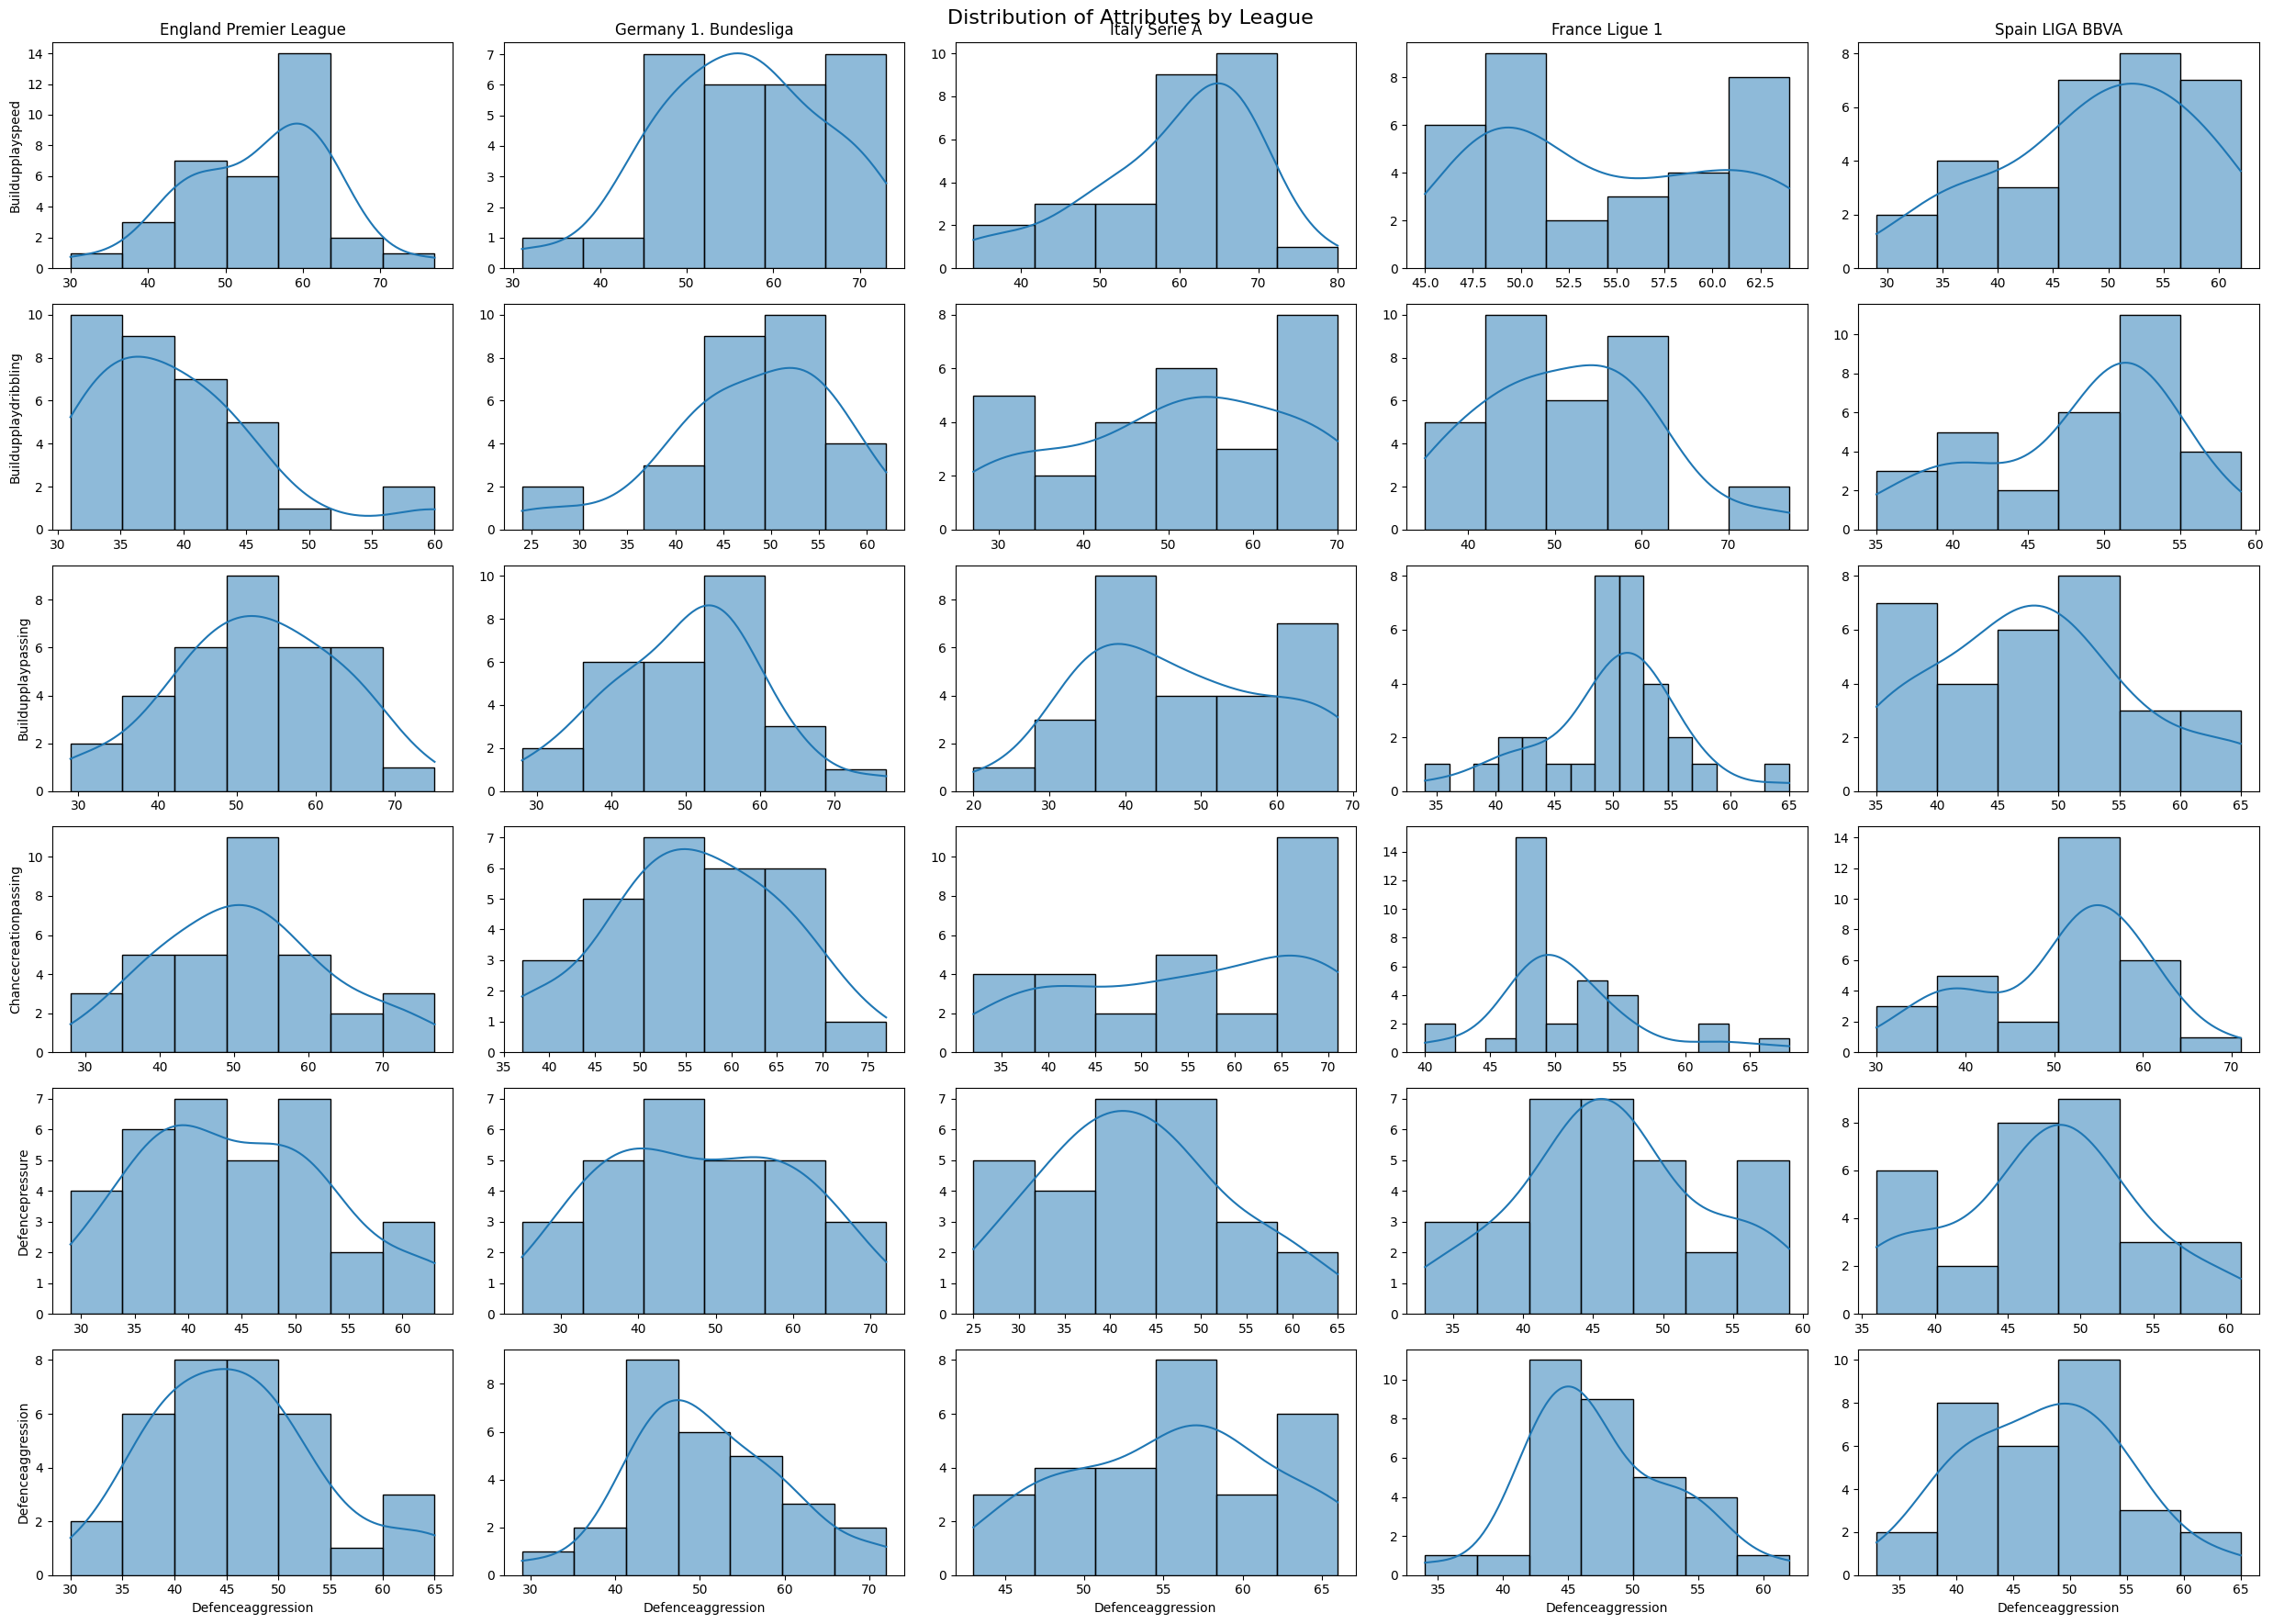
\includegraphics[width=0.7\linewidth]{league_features.png}
    \caption{Leagues Based Team Characteristics}
    \label{fig:enter-label}
\end{figure}

\begin{figure}
    \centering
    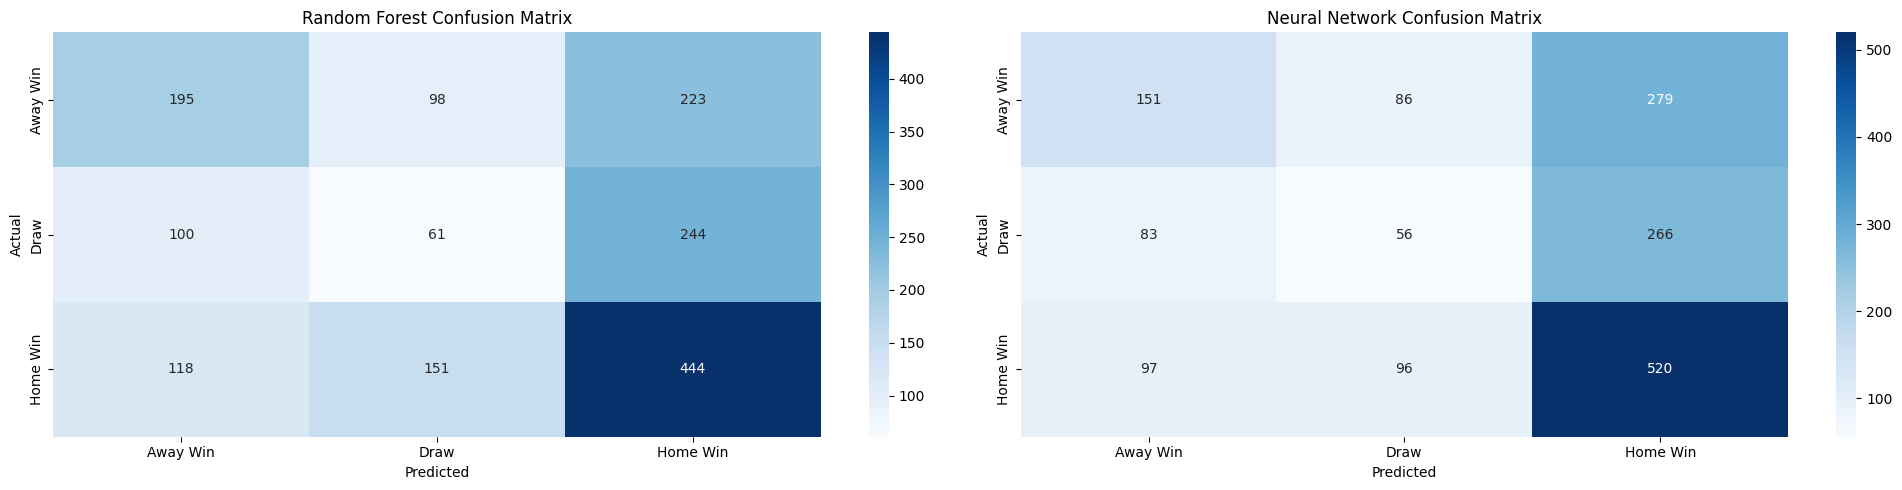
\includegraphics[width=0.8\linewidth]{ConfusionMatrix.png}
    \caption{Confusion Matrices}
    \label{fig:enter-label}
\end{figure}
\section{Conclusion}
The code is available in the GitHub repository \href{https://github.ncsu.edu/arao23/engr-ALDA-Fall2024-P28}{here}.
.We have preliminary results for the match prediction task, showing that Neural Networks outperform Random Forest classifiers due to their ability to capture underlying data patterns without significant overfitting. To enhance our predictions, we can improve feature selection, handle missing values more effectively, and expand the dataset by including matches from 2008 to 2014. Additionally, we found that ensemble methods can deliver accuracy comparable to Neural Networks while requiring lower computational costs. Thus, we will also explore ensembling various classifiers alongside Random Forests for better results.

The exploratory data analysis (EDA) has highlighted key features and their relevance for different roles within a team. Our next steps involve selecting a specific team to identify weaknesses in its attacking and defensive structure. We will then pinpoint players who can address these gaps, either by filtering based on specific requirements or by targeting promising upcoming players with strong career trajectories in the needed areas. To forecast how these players will perform, we will utilize regression analysis. This helps us in picking players from lower leagues or players who are young and will hit their peak form.

\section{References}

\small{


[1] Ulmer, Ben, Matthew Fernandez, and Michael Peterson. "Predicting soccer match results in the English premier league." Doctoral dissertation, Doctoral dissertation, Ph. D. dissertation, Stanford (2013).


[2] Shin, J., \& Gasparyan, R. (2014). A novel way to soccer match prediction. Stanford University: Department of Computer Science.


[3] Luca Pappalardo, Paolo Cintia, Paolo Ferragina, Emanuele Massucco, Dino Pedreschi, and Fosca Giannotti. 2019. PlayeRank: Data-driven Performance Evaluation and Player Ranking in Soccer via a Machine Learning Approach. ACM Trans. Intell. Syst. Technol. 10, 5, Article 59 (September 2019), 27 pages. https://doi.org/10.1145/3343172
}
\normalsize
% \appendix
% \section{Plan of Activities}
% One of us will focus on improving the current results with Random Forest and Neural Networks. The remaining members will work on extracting information and prediction for the transfer analysis part.

% \section{Second Appendix}
% This is the second appendix.
\end{document}

